\documentclass[a4paper,12pt]{article} 


\usepackage[T2A]{fontenc}			
\usepackage[utf8]{inputenc}			
\usepackage[english,russian]{babel}	

\usepackage{graphicx, scalerel}    
\usepackage{wrapfig}               
\usepackage[14pt]{extsizes}        
\usepackage[warn]{mathtext}       
\usepackage{indentfirst}      
\usepackage[margin = 25mm]{geometry}
\usepackage[table,xcdraw]{xcolor} 
\usepackage{amsmath,amsfonts,amssymb,amsthm,mathtools}
\usepackage{wasysym}                
\usepackage{upgreek}                
\usepackage{caption}
\usepackage{multirow}
\captionsetup{labelsep=period}
\usepackage[font=small,labelfont=bf]{caption}
\usepackage{gensymb}
\usepackage{icomma}

\usepackage[unicode, pdftex]{hyperref}
\usepackage{tikz}
\usetikzlibrary{positioning}
\usepackage{fancyhdr}
\pagestyle{fancy}
\setlength\fboxsep{3pt} % Отступ рамки \fbox{} от рисунка
\setlength\fboxrule{1pt} % Толщина линий рамки \fbox{}
\usepackage{tocloft}
\newcommand{\tocsection}[1]{\section*{#1} \addcontentsline{toc}{section}{#1}}
\newcommand{\tocsubsection}[1]{\subsection*{#1} \addcontentsline{toc}{subsection}{#1}}
\renewcommand{\cftsecleader}{\cftdotfill{\cftdotsep}}

\begin{document}
	\newcommand{\HRule}{\rule{\linewidth}{0.7mm}} % Defines a new command for the horizontal lines, change thickness here

\begin{center}
	\large\textbf{Московский Физико-Технический Институт}\\
	\large\textbf{(государственный университет)}
	
	\vfill
	
	
	
	\Large Лабораторная работа 5.1.2
	%----------------------------------------------------------------------------------------
	%	TITLE SECTION
	%----------------------------------------------------------------------------------------
	
	\HRule
	\\[0.4cm]
	{ \huge \bfseries Исследование эффекта Комптона}
	\\[0.4cm] % Title of your document
	\HRule
	\\[0.5cm]
	
	\ \\
	\textbf{\large Автор:} \\	
	\large Овсянников Михаил Б01-008\\
	\vfill
	\hspace*{-0.8 cm}
\includegraphics[width=100 pt]{./Include/frkt_logo.pdf}\\
	\large Долгопрудный, 2022
\end{center}

\thispagestyle{empty}

\newpage
\setcounter{page}{2}
\fancyfoot[c]{\thepage}
\fancyhead[L] {Лабораторная работа 5.1.2}
\fancyhead[R] {Исследование эффекта Комптона}

	\newpage
	
	\tableofcontents
	
	
	
	\newpage
	\textbf{Цель работы:} С помощью сцинтилляционного счетчика измеряются линейные коэффициенты ослабления потока $\gamma$-лучей в свинце, железе и алюминии; по их величине определяется энергия $\gamma$-квантов.

	\tocsection{Теоретические сведения}
	Гамма-лучи возникают при переходе возбужденных ядер из одного энергетического состояния в другое, более низкое. Проходя через вещество, пучок $\gamma$-квантов постепенно ослабляется. Ослабление происходит по экспоненциальному закону, который может быть записан в двух эквивалентных формах:
	\begin{equation}
		I = I_0 e^{-\mu l};
	\end{equation}
	\begin{equation}
		I = I_0 e^{-\mu' m_1}.
	\end{equation}

	В этих формулах $I$, $I_0$ -- интенсивности прошедшего и падающего излучений, $l$ -- длина пути, пройденного пучком $\gamma$-лучей, $m_1$ -- масса пройденного вещества, приходящаяся на единицу площади, $\mu$ и $\mu'$ -- константы, величина которых зависит от вещества, сквозь которое проходят $\gamma$-лучи.
	
	Ослабление потока $\gamma$-лучей, происходящее при прохождении среды, связано с тремя эффектами: фотоэлектрическим поглощением, комптоновским рассеянием и с генерацией электрон-позитронных пар.
	
	
	\textbf{Фотоэлектрическое поглощение.} При столкновении $\gamma$-квантов с электронами внутренних атомных оболочек может происходить поглощение квантов. Энергия $\gamma$-кванта передается соответствующему электрону, а импульс делится между этим электроном и оставшимся после его вылета ионом. Свободный электрон не может поглотить $\gamma$-квант, так как при этом невозможно одновременно удовлетворить законам сохранения энергии и импульса. Наружные электроны не принимают участия в фотоэлектрическом поглощении, потому что они слабо связаны в атоме, так что их практически можно считать свободными. Фотоэффект является доминирующим механизмом поглощения $\gamma$-квантов при не очень высоких энергиях.

	
	
	
	\textbf{Комптоновское рассеяние.} Комптоновским рассеянием (или комптон-эффектом) называется упругое столкновение $\gamma$-кванта с электроном. При таком столкновении $\gamma$-квант передает электрону часть своей энергии, величина которой определяется углом рассеяния. В отличие от фотоэффекта, который может идти только на сильно связанных электронах, комптоновское рассеяние происходит на свободных или слабосвязанных электронах. Роль эффекта Комптона становится существенной только тогда, когда энергия квантов становится много больше энергии связи электронов в атоме. В отличие от фотоэффекта, эффект Комптона приводит не к поглощению $\gamma$-квантов, а к их рассеянию и уменьшению их энергии.

	
	
	\textbf{Образование пар.} При энергиях $\gamma$-лучей, превышающих $2mc^2 = 1,02$ МэВ, становится возможен процесс поглощения $\gamma$-лучей, связанный с образованием электрон-позитронных пар. Рождение пар не может происходить в вакууме, оно возникает в электрическом поле ядер. При энергиях больше $2mc^2$ фотоэффект даже для самых тяжелых ядер уже не играет практически никакой роли. Вероятность образования пар должна поэтому сравниваться с вероятностью комптоновского рассеяния. При энергиях, с которыми приходится иметь дело при изучении ядер, рождение пар существенно только в самых тяжелых элементах.
	
	
	\textbf{Полный коэффициент ослабления потока $\gamma$-лучей.} Полный линейный коэффициент $\mu$ ослабления пучка $\gamma$-квантов при прохождении через вещество равен сумме коэффициентов для всех трех рассмотренных процессов.
	
	
	
	В данной работе измеряется коэффициент ослабления $\mu$.
	\begin{equation}
		\mu = \frac{1}{l} \ln \frac{N_0}{N}
	\end{equation}
	Для определения коэффициента ослабления нужно, таким образом, измерить толщину образца $l$, число падающих частиц $N_0$ и число частиц $N$, прошедших через образец.
	
	\tocsection{Экспериментальная установка}
	Схема установки, используемой в работе, показана на рис. \ref{WeakCoeff_Scheme}.
	\begin{figure}[h!]
		\centering
		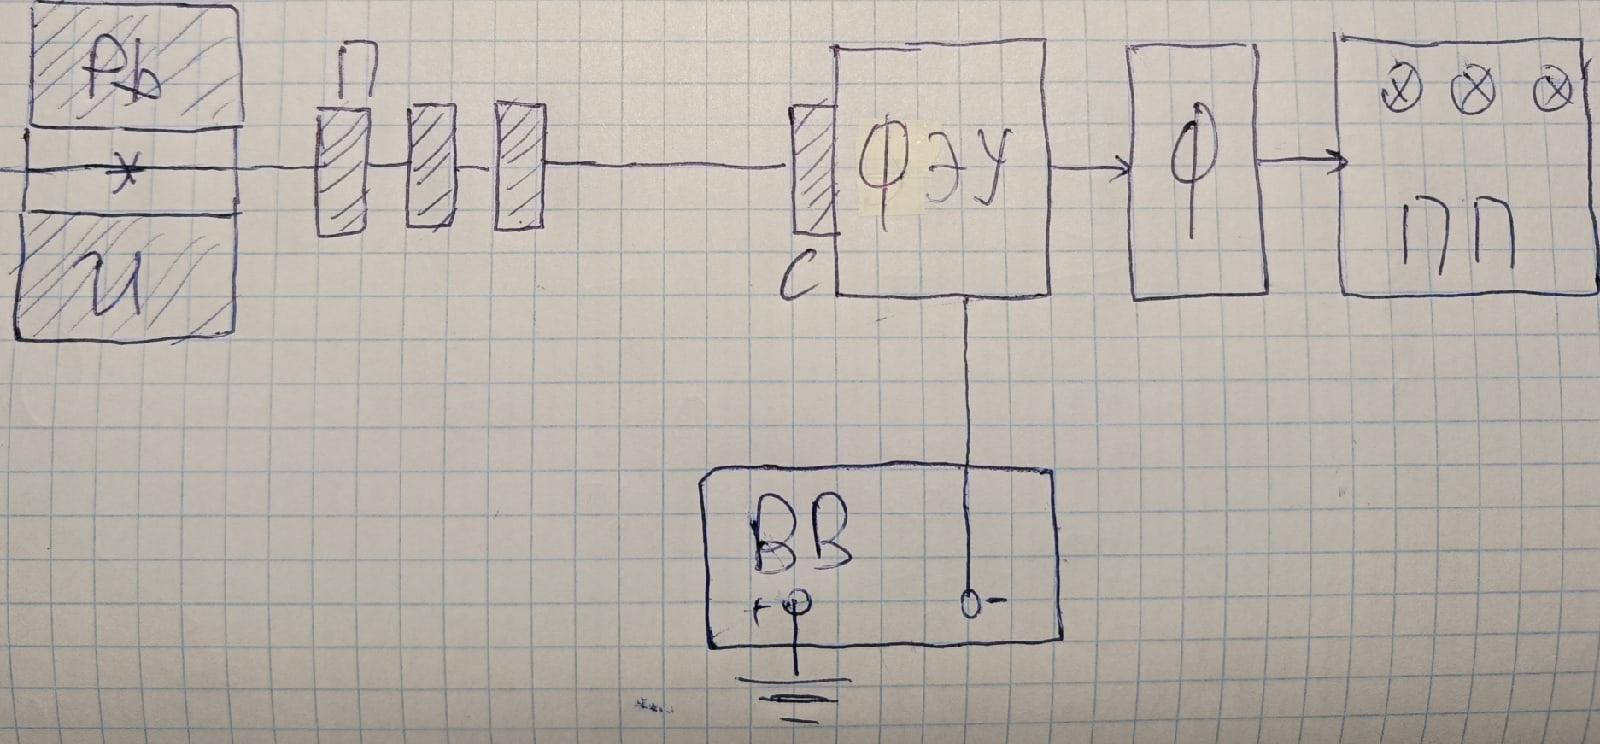
\includegraphics[width=0.8\linewidth]{Pictures/Scheme}
		\caption{Экспериментальная установка}
		\label{WeakCoeff_Scheme}
	\end{figure}
	Свинцовый коллиматор выделяет узкий почти параллельный пучок $\gamma$-квантов, проходящий через набор поглотителей П и регистрируемый сцинтилляционным счетчиком. Сигналы от счетчика усиливаются и регистрируются пересчетным прибором ПП. Высоковольтный выпрямитель ВВ обеспечивает питание сцинтилляционного счетчика.

	
	
	\tocsection{Ход работы}
	\begin{enumerate}
		\item Включим пересчетный прибор и высоковольтный выпрямитель.
		
		\item Убедимся в том, что установка работает. Для этого подадим на ФЭУ напряжение, указанное на установке. Измерим скорость счета при полностью открытом коллиматоре, а затем при коллиматоре, закрытом свинцовой пробкой. Скорость счета резко уменьшилась, значит действительно, установка работает, как следует.
		
		\item Исследуем поглощение $\gamma$-лучей в свинце, железе и алюминии. Измерим поглощение $\gamma$-лучей при различных толщинах образцов.
		
		При проведении эксперимента с $n$ пластинами конкретного металла использовались $n-1$ пробок, чередующих эти пластины. Именно поэтому в каждом эксперименте с $n$ пластинами за $N_0$ следует считать то, что было зафиксировано при $n-1$ пробках без какого-либо металла. 
		
		Количество частиц считается за 10 секунд. Результаты занесем в таблицу \ref{WeakCoeff_Table}.
		
		На данном этапе мы уже можем посчитать коэффициенты ослабления для каждого из экспериментов и их погрешности.
		Поскольку
		\begin{equation*}
			\mu = \frac{1}{l}\ln \frac{N_0}{N},
		\end{equation*}
		\noindent то
		\begin{equation*}
			\sigma_\mu = \frac{1}{l}\sqrt{\mu^2 \sigma_l^2 + \frac{\sigma_{N_0}^2}{N_0^2} + \frac{\sigma_N^2}{N^2}}
		\end{equation*}
	
		Погрешность штангенциркуля $\sigma_l = 0,1$ мм $= 0,01$ см.
		
		Погрешности числа частиц $\sigma_N = \sqrt{N}$. То же и для $N_0$.
		
		Предварительно посчитаем значения коэффициентов ослабления в каждом опыте и их погрешности. Занесем их в таблицу \ref{WeakCoeff_PreTable}.
		

		\begin{table}[h!]
			\centering
			\resizebox{\columnwidth}{!}{%
				\begin{tabular}{|rrcc|rrrllrrr}
					\cline{1-4} \cline{11-12}
					\multicolumn{1}{|r|}{Количество пластин} & \multicolumn{1}{c|}{$l$, см} & \multicolumn{1}{c|}{$N_1$} & $N_2$ &  &  &  &  &  & \multicolumn{1}{r|}{} & \multicolumn{2}{c|}{Пробки}                                          \\ \cline{1-4} \cline{11-12} 
					\multicolumn{4}{|c|}{Свинец}                                                                                 &  &  &  &  &  & \multicolumn{1}{r|}{} & \multicolumn{1}{r|}{Количество пробок} & \multicolumn{1}{c|}{$N$}    \\ \cline{1-4} \cline{11-12} 
					\multicolumn{1}{|r|}{1}                  & \multicolumn{1}{r|}{0,49}    & \multicolumn{1}{c|}{74415} & 75164 &  &  &  &  &  & \multicolumn{1}{r|}{} & \multicolumn{1}{r|}{0}                 & \multicolumn{1}{l|}{139843} \\ \cline{1-4} \cline{11-12} 
					\multicolumn{1}{|r|}{2}                  & \multicolumn{1}{r|}{0,97}    & \multicolumn{1}{c|}{41098} & 42065 &  &  &  &  &  & \multicolumn{1}{r|}{} & \multicolumn{1}{r|}{1}                 & \multicolumn{1}{l|}{136826} \\ \cline{1-4} \cline{11-12} 
					\multicolumn{1}{|r|}{3}                  & \multicolumn{1}{r|}{1,45}    & \multicolumn{1}{c|}{23371} & 23489 &  &  &  &  &  & \multicolumn{1}{r|}{} & \multicolumn{1}{r|}{2}                 & \multicolumn{1}{l|}{133850} \\ \cline{1-4} \cline{11-12} 
					\multicolumn{1}{|r|}{4}                  & \multicolumn{1}{r|}{1,90}    & \multicolumn{1}{c|}{13985} & 13987 &  &  &  &  &  & \multicolumn{1}{r|}{} & \multicolumn{1}{r|}{3}                 & \multicolumn{1}{l|}{131576} \\ \cline{1-4} \cline{11-12} 
					\multicolumn{1}{|r|}{5}                  & \multicolumn{1}{r|}{2,35}    & \multicolumn{1}{c|}{8452}  & 8251  &  &  &  &  &  & \multicolumn{1}{r|}{} & \multicolumn{1}{r|}{4}                 & \multicolumn{1}{l|}{129176} \\ \cline{1-4} \cline{11-12} 
					\multicolumn{4}{|c|}{Железо}                                                                                 &  &  &  &  &  &                       &                                        &                             \\ \cline{1-4}
					\multicolumn{1}{|r|}{1}                  & \multicolumn{1}{r|}{1,01}    & \multicolumn{1}{c|}{77976} & 77286 &  &  &  &  &  &                       &                                        &                             \\ \cline{1-4}
					\multicolumn{1}{|r|}{2}                  & \multicolumn{1}{r|}{2,04}    & \multicolumn{1}{c|}{42158} & 40827 &  &  &  &  &  &                       &                                        &                             \\ \cline{1-4}
					\multicolumn{1}{|r|}{3}                  & \multicolumn{1}{r|}{3,02}    & \multicolumn{1}{c|}{23599} & 23808 &  &  &  &  &  &                       &                                        &                             \\ \cline{1-4}
					\multicolumn{1}{|r|}{4}                  & \multicolumn{1}{r|}{4,03}    & \multicolumn{1}{c|}{13315} & 13294 &  &  &  &  &  &                       &                                        &                             \\ \cline{1-4}
					\multicolumn{1}{|r|}{5}                  & \multicolumn{1}{r|}{5,03}    & \multicolumn{1}{c|}{7667}  & 7552  &  &  &  &  &  &                       &                                        &                             \\ \cline{1-4}
					\multicolumn{4}{|c|}{Алюминий}                                                                               &  &  &  &  &  &                       &                                        &                             \\ \cline{1-4}
					\multicolumn{1}{|r|}{1}                  & \multicolumn{1}{r|}{2,01}    & \multicolumn{1}{c|}{90864} & 89504 &  &  &  &  &  &                       &                                        &                             \\ \cline{1-4}
					\multicolumn{1}{|r|}{2}                  & \multicolumn{1}{r|}{4,02}    & \multicolumn{1}{c|}{58396} & 58788 &  &  &  &  &  &                       &                                        &                             \\ \cline{1-4}
					\multicolumn{1}{|r|}{3}                  & \multicolumn{1}{r|}{5,99}    & \multicolumn{1}{c|}{38139} & 38010 &  &  &  &  &  &                       &                                        &                             \\ \cline{1-4}
					\multicolumn{1}{|r|}{4}                  & \multicolumn{1}{r|}{7,99}    & \multicolumn{1}{c|}{24878} & 24118 &  &  &  &  &  &                       &                                        &                             \\ \cline{1-4}
					\multicolumn{1}{|r|}{5}                  & \multicolumn{1}{r|}{10,02}   & \multicolumn{1}{c|}{16626} & 16524 &  &  &  &  &  &                       &                                        &                             \\ \cline{1-4}
				\end{tabular}%
			}
		\caption{Результаты экспериментов}
		\label{WeakCoeff_Table}
		\end{table}
		\begin{table}[h!]
			\centering
			\begin{tabular}{|rrll|}
				\hline
				\multicolumn{1}{|r|}{Количество пластин} & \multicolumn{3}{c|}{$\mu$, см$^{-1}$}  \\ \hline
				\multicolumn{4}{|c|}{Свинец}                                                      \\ \hline
				\multicolumn{1}{|r|}{1}                  & \multicolumn{3}{r|}{$1,28 \pm 0,03$}   \\ \hline
				\multicolumn{1}{|r|}{2}                  & \multicolumn{3}{r|}{$1,23 \pm 0,02$}   \\ \hline
				\multicolumn{1}{|r|}{3}                  & \multicolumn{3}{r|}{$1,20 \pm 0,01$}   \\ \hline
				\multicolumn{1}{|r|}{4}                  & \multicolumn{3}{r|}{$1,18 \pm 0,01$}   \\ \hline
				\multicolumn{1}{|r|}{5}                  & \multicolumn{3}{r|}{$1,17 \pm 0,01$}   \\ \hline
				\multicolumn{4}{|c|}{Железо}                                                      \\ \hline
				\multicolumn{1}{|r|}{1}                  & \multicolumn{3}{r|}{$0,583 \pm 0,007$} \\ \hline
				\multicolumn{1}{|r|}{2}                  & \multicolumn{3}{r|}{$0,585 \pm 0,004$} \\ \hline
				\multicolumn{1}{|r|}{3}                  & \multicolumn{3}{r|}{$0,573 \pm 0,003$} \\ \hline
				\multicolumn{1}{|r|}{4}                  & \multicolumn{3}{r|}{$0,569 \pm 0,003$} \\ \hline
				\multicolumn{1}{|r|}{5}                  & \multicolumn{3}{r|}{$0,563 \pm 0,003$} \\ \hline
				\multicolumn{4}{|c|}{Алюминий}                                                    \\ \hline
				\multicolumn{1}{|r|}{1}                  & \multicolumn{3}{r|}{$0,218 \pm 0,002$} \\ \hline
				\multicolumn{1}{|r|}{2}                  & \multicolumn{3}{r|}{$0,211 \pm 0,001$} \\ \hline
				\multicolumn{1}{|r|}{3}                  & \multicolumn{3}{r|}{$0,210 \pm 0,001$} \\ \hline
				\multicolumn{1}{|r|}{4}                  & \multicolumn{3}{r|}{$0,210 \pm 0,001$} \\ \hline
				\multicolumn{1}{|r|}{5}                  & \multicolumn{3}{r|}{$0,205 \pm 0,001$} \\ \hline
			\end{tabular}
		\caption{Предварительно посчитанные $\mu$}
		\label{WeakCoeff_PreTable}
		\end{table}
	
	
	
	\end{enumerate}	
	\newpage
	Теперь построим график зависимости $\ln \frac{N_0}{N}$ от $l$ и по коэффициенту наклона определим значение $\mu$.
	
	\begin{figure}[h!]
		\centering
		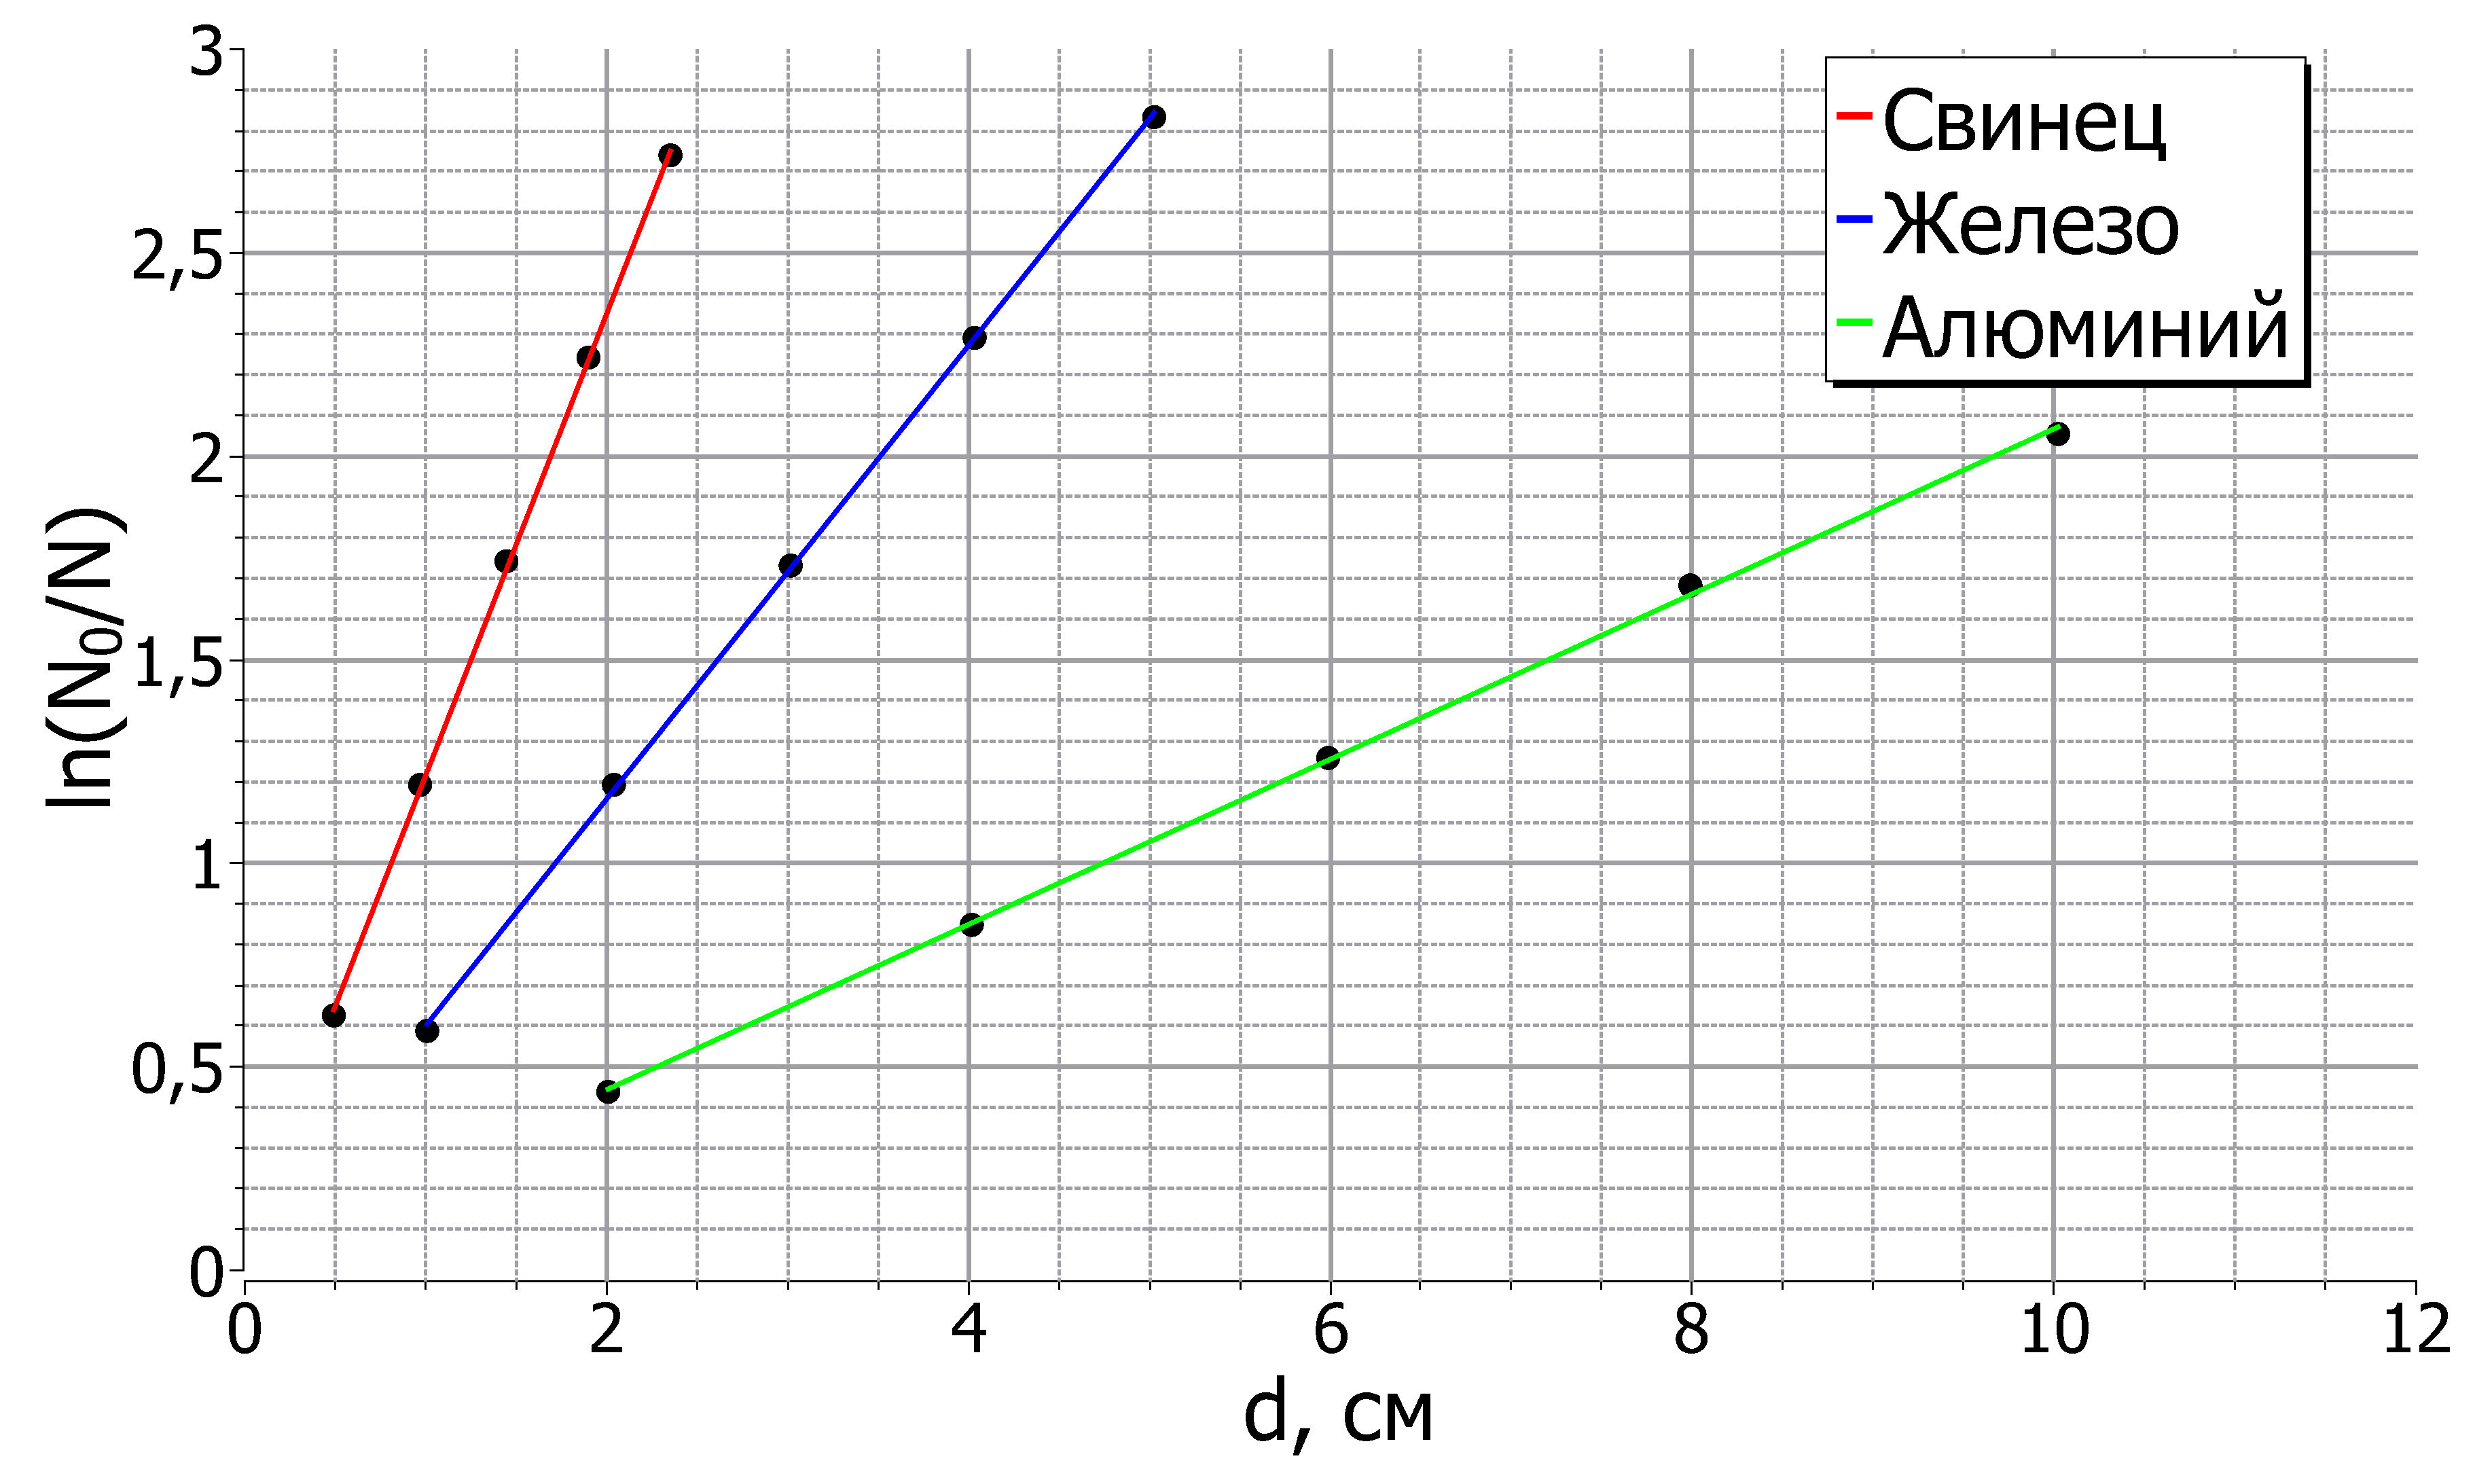
\includegraphics[width=\linewidth]{Pictures/Plot.pdf}
		\caption{Зависимости $\ln \frac{N_0}{N}$ от $d$ для трех материалов}
	\end{figure}

	Из этих графиков мы получаем:
	\begin{itemize}
		\item Для свинца $\mu = (1,14 \pm 0,01)$ см$^{-1}$
		
		\item Для железа $\mu = (0,557 \pm 0,005)$ см$^{-1}$
		
		\item Для алюминия $\mu = (0,198 \pm 0,003)$ см$^{-1}$
	\end{itemize}
	Если пересчитать в $\mu'$, то получаем:
	\begin{itemize}
		\item Для свинца $\rho = 11,35$ г/см$^3$ \;\;\;\,$\Longrightarrow$ $\mu' = (0,100 \pm 0,001)$ см$^2$/г
		
		\item Для железа $\rho = 7,87$ г/см$^3$ \;\;\;\;\;$\Longrightarrow$ $\mu' = (0,071 \pm 0,001)$ см$^2$/г
		
		\item Для алюминия $\rho = 2,70$ г/см$^3$ $\Longrightarrow$ $\mu' = (0,073 \pm 0,001)$ см$^2$/г
	\end{itemize}

	Используя табличные данные, найдем среднюю энергию $\gamma$-частиц.
	
	\begin{itemize}
		\item Для свинца получаем $E_\gamma = 0,70$ МэВ 
		
		\item Для железа получаем $E_\gamma = 0,70$ МэВ
		
		\item Для алюминия получаем $E_\gamma = 0,69$ МэВ
	\end{itemize}

	
	\newpage
	\tocsection{Вывод}
	В данной работе мы измерили коэффициенты ослабления потока $\gamma$-лучей в трех различных материалах таких как свинец, железо и алюминий. Были измерены коэффициенты как линейные $\mu$, так и нормированные на плотность вещества $\mu'$.
	\begin{table}[h!]
		\centering
			\begin{tabular}{c|c|c|}
				\cline{2-3}
				& $\mu$, см$^{-1}$    & $\mu'$, см$^2$/г    \\ \hline
				\multicolumn{1}{|c|}{Свинец}   & $(1,14 \pm 0,01)$   & $(0,100 \pm 0,001)$ \\ \hline
				\multicolumn{1}{|c|}{Железо}   & $(0,557 \pm 0,005)$ & $(0,071 \pm 0,001)$ \\ \hline
				\multicolumn{1}{|c|}{Алюминий} & $(0,198 \pm 0,003)$ & $(0,073 \pm 0,001)$ \\ \hline
			\end{tabular}
		\caption{Сводная таблица}
	\end{table}
	Как видим, некоторые ошибки присутствуют, однако они все не больше $1,5\%$. Помимо этого всего, в работе была рассчитана средняя энергия $\gamma$-лучей, испускаемых источником на данной установке: $E_\gamma = 0,7$ МэВ.
	
\end{document}